
\documentclass[../Thesis.tex]{subfiles}
\graphicspath{{\subfix{../figures/}}}
\begin{document}
\chapter{Appendix}

\section{Suicide data}
\begin{table}[H]
    \centering
    \begin{tabular}{cccccc}
1 & 25 & 40 & 83 & 123 & 256 \\
1 & 27 & 49 & 84 & 126 & 257 \\
1 & 27 & 49 & 84 & 129 & 311 \\
5 & 30 & 54 & 84 & 134 & 314 \\
7 & 30 & 56 & 90 & 144 & 322 \\
8 & 31 & 56 & 91 & 147 & 369 \\
8 & 31 & 62 & 92 & 153 & 415 \\
13 & 32 & 63 & 93 & 163 & 573 \\
14 & 34 & 65 & 93 & 167 & 609 \\
14 & 35 & 65 & 103 & 175 & 640 \\
17 & 36 & 67 & 103 & 228 & 737 \\
18 & 37 & 75 & 111 & 231 \\
21 & 38 & 76 & 112 & 235 \\
21 & 39 & 79 & 119 & 242 \\
22 & 39 & 82 & 122 & 256
    \end{tabular}
    \caption{The length of treatment of control patients in suicide study. The data originates from the Mental Health Enquiry (MHE) of England of Wales and was published in 1967.}
    \label{tab:suicide data}
\end{table}

\newpage
\section{Confidence interval for absolute correlation in bivariate Gaussian}\label{sec:bivar gauss abs correlation CI}
From \cite{Confidence_in_Correlation}, given a bivariate Gaussian, the confidence distribution of $\rho$ given the empirical correlation $r$ based on $n$ observations is given by
$$f\left(\rho \mid r,\nu\right) = \frac{\nu (\nu-1) \Gamma(\nu-1)}{\sqrt{2\pi} \Gamma(\nu + \frac{1}{2})} \frac{\left(1-r^2\right)^{\frac{\nu-1}{2}} \left(1-\rho^2\right)^{\frac{\nu-2}{2}} }{\left(1-r\rho\right)^{\frac{2\nu-1}{2}}} F\left(\frac{3}{2}, -\frac{1}{2}, \nu+\frac{1}{2}, \frac{1+r\rho}{2}\right)$$
where $F\left(a,b,c,z\right)$ is the Gaussian hypergeometric function and $\nu = n-1$. That is, given a sample correlation $r$, what is the confidence in $\rho$ in terms of a distribution. In the following figure, a sample correlation $r=0.8$ and $r=0$ has been used with varying number of observations (degrees of freedom) in figures \autoref{subfig:gaussian correlation dist 0.8} and \autoref{subfig:gaussian correlation dist 0} respectively.
\begin{figure}[h]
    \centering
    \begin{subfigure}[t]{0.49\linewidth}
        \centering
        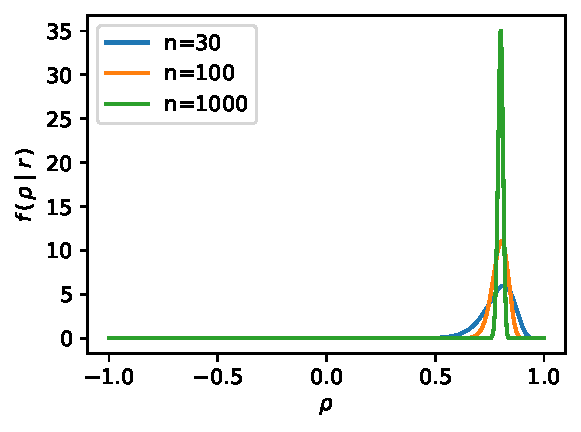
\includegraphics[width=\linewidth]{figures/Gaussian correlation confidence dist/density comparison r 0.8.pdf}
        \caption{}
        \label{subfig:gaussian correlation dist 0.8}
    \end{subfigure}%
    ~
    \begin{subfigure}[t]{0.49\linewidth}
        \centering
        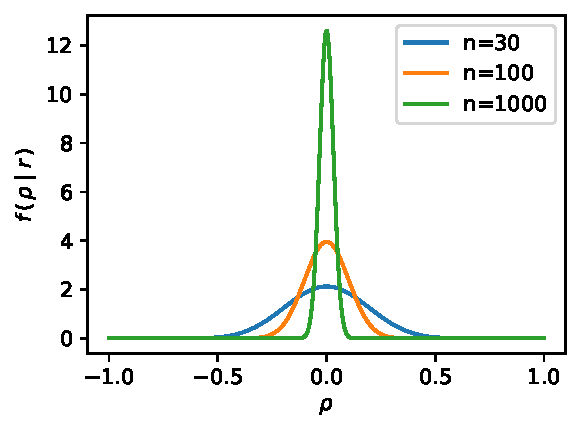
\includegraphics[width=\linewidth]{figures/Gaussian correlation confidence dist/density comparison r 0.pdf}
        \caption{}
        \label{subfig:gaussian correlation dist 0}
    \end{subfigure}
    \caption{$f\left(\rho \mid r, \nu\right)$ shown for $r=0.8$ and $r=0$ in (a) and (b) with $n\in \{30,100,1000\}$. As one would expect, the power i.e. the width of the peak decreases with increasing n and for correlations closer to $0$, the width is the largest.}
\end{figure}
A key property is that $f$ is \textit{even symmetric} in $\rho,\, r$. That is $f(\rho \mid r) = f(-\rho \mid -r)$. Thus, a confidence interval for $\rho$ given $r$ is the negative of the confidence interval given $-r$. In particular, if we only observe $|r|$, we can calculate a confidence interval for $\rho$ up to the sign of the bounds of the interval. Furthermore, as we want a CI for $|\rho|$, it does not matter if $r$ is negative or positive. Hence, without loss of generality, we assume that $r \geq 0$. At this point, to construct a confidence interval for $|\rho|$ we list the following desired properties. Firstly, it should be an exact confidence interval, meaning that for a given significance level $\alpha$, the CI includes the true value exactly $1-\alpha$ fraction of the times. Secondly, if for a given $r$, it can not be rejected that $\rho$ is 0, 0 should also be contained in the interval. Finally, if we reject that $\rho = 0$, we shall have $\alpha/2$ probability mass above and below the bounds of the interval. The above is enough to uniquely define a confidence interval in all cases. Before continuing with how this CI is calculated, we mention that as $r$ is an unbiased estimator of $\rho$, we would preferably want $|r| \in CI_{1-\alpha}\left(|\rho|\right)$ (where $CI_{1-\alpha}\left(|\rho|\right)$ denotes the $1-\alpha$ confidence interval for $|\rho|$). However, although this will in almost every scenario be the case, we can not be sure of this from the above properties and in fact examples with large $\alpha$ can be constructed such that $|r|$ lies just outside the constructed CI.

First, to conform with the second desired property, if it can not be rejected that $\rho = 0$ on a significance level $\alpha$, we will initially compute a CI for $\rho$ (not $|\rho|$) based on $r$ (wlog chosen to be non-negative). This CI will just be a symmetric CI in the sense that $\alpha/2$ of the probability mass will lie below the lower bound of the CI and above the upper bound of the CI respectively. If $0$ is contained in this CI, we can not reject that $\rho=0$ and vice versa on an $\alpha$ significance level. Thus, if $0$ is contained in this initial CI for $\rho$, we will start the CI for $|\rho|$ at $0$ and determine and upper bound $b$ such that $\alpha$ probability mass is above this $b$. Otherwise, we shall find $a$ and $b$ such that $\alpha/2$ probability mass is below $a$ and above $b$ respectively. Choosing $a$ and $b$ this way also conforms with the third property. Finally, to ensure that the CI contains exactly $1-\alpha$, we define $\tilde{f}$ as the reflected $f$ in $\rho$ such that
$$\tilde{f}\left(\rho_a \mid r_a, \nu\right) = f(\rho_a \mid r_a, \nu) + f(-\rho_a \mid r_a, \nu),\quad \rho_a,r \in [0,1]$$
where $\rho_a$ and $r_a$ is the absolute correlation and empirical correlation respectively. With this $\tilde{f}$, the density at $\rho_a$ is both the density for the negative and positive correlation ensuring that the $\tilde{f}$ has probability mass $1$. Thus, if $a=0$ (i.e. the CI must contain $0$), we find $b$ as the $1-\alpha$ percentile of $\tilde{f}$ and if $a\neq 0$, we take $a$ as the $\alpha/2$ percentile and $b$ as the $1-\alpha/2$ percentile of $\tilde{f}$.

As an example, suppose $r_a=0.06$ with $1000$ observations. Then a $95\%$ CI for $|\rho|$ is $[0, 0.11164]$ whereas if on had observed $r_a = 0.07$ the CI would be $[0.01071, 0.1314]$. These CI could then be used to test the absolute correlation of a bivariate Gaussian i.e. for $r_a = 0.07$ based on $1000$ observations would be rejected as stemming from a Gaussian with absolute correlation $0.01$ on a $5\%$ significance level.


\newpage
\section{Gaussian chain deconvolution}

\begin{figure}[H]
    \centering
    \begin{subfigure}[t]{0.49\textwidth}
        \centering
        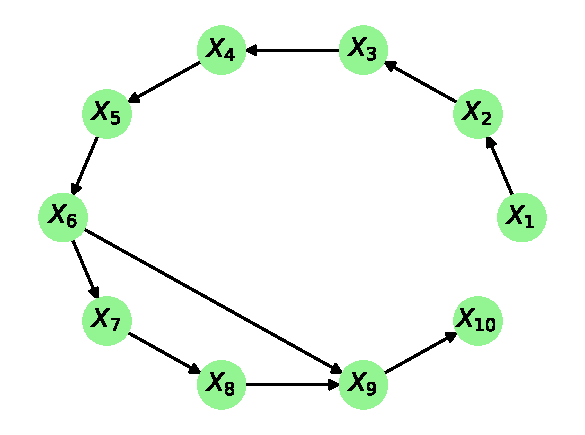
\includegraphics[width=.95\linewidth]{figures/Gaussian Chain Theoretical/Chain graph from triangular G obs - MI - cutoff 2e-2.pdf}
        \caption{}
        % \label{fig:Gaussian 3x3 large s}
    \end{subfigure}
    \hfill
    \begin{subfigure}[t]{0.49\textwidth}
        \centering
        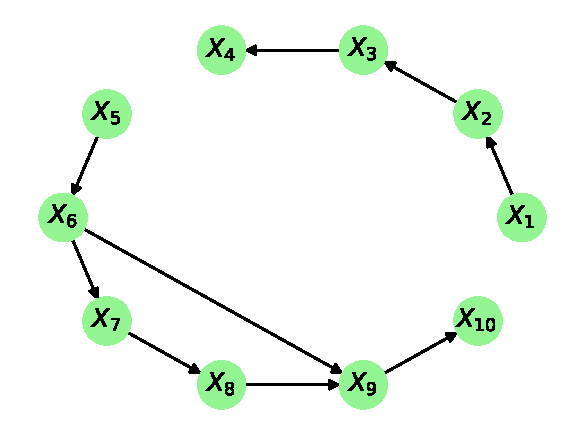
\includegraphics[width=.95\linewidth]{figures/Gaussian Chain Theoretical/Chain graph from triangular G obs - MI - cutoff 2_1e-2.pdf}
        \caption{}
        % \label{fig:Gaussian 3x3 large s}
    \end{subfigure}
    \\[\baselineskip]
    \begin{subfigure}[t]{0.49\textwidth}
        \centering
        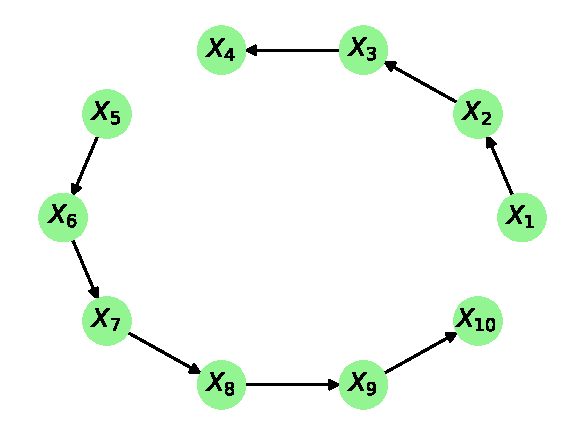
\includegraphics[width=.95\linewidth]{figures/Gaussian Chain Theoretical/Chain graph from triangular G obs - MI - cutoff 4_51e-2.pdf}
        \caption{}
        % \label{fig:Gaussian 3x3 large s}
    \end{subfigure}
    \caption{Triangular, mutual information, cutoff $2\cdot 10^{-10}$, $2.1 \cdot 10^{-2}$ and $4.51 \cdot 10^{-2}$.}
    \label{fig:Gaussian chain symmetric G_obs using mutual information different cutoff}
\end{figure}


\newpage
\section{Gaussian network deconvolution}
\begin{figure}[H]
    \centering
    \begin{subfigure}[t]{0.49\textwidth}
        \centering
        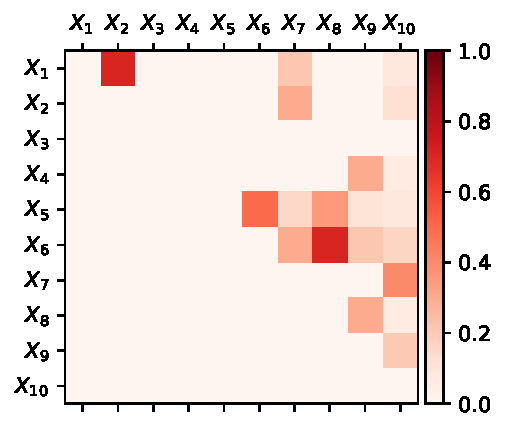
\includegraphics[width=.95\linewidth]{figures/Gaussian Network Theoretical/triangular G obs - cor.pdf}
        \caption{$G_{obs}$}
        % \label{fig:Gaussian 3x3 large s}
    \end{subfigure}
    \hfill
    \begin{subfigure}[t]{0.49\textwidth}
        \centering
        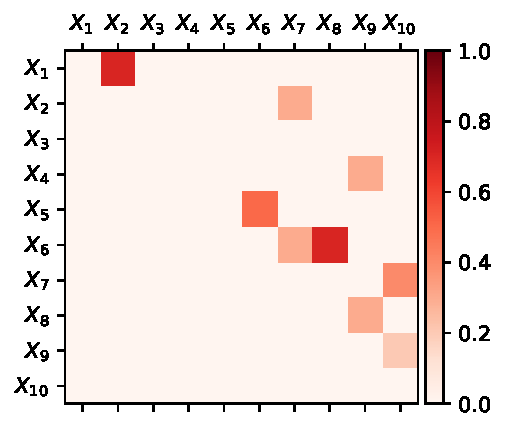
\includegraphics[width=.95\linewidth]{figures/Gaussian Network Theoretical/G dir from triangular G obs - cor.pdf}
        \caption{$G_{dir}$}
        % \label{fig:Gaussian 3x3 large s}
    \end{subfigure}
    \\[\baselineskip]
    \begin{subfigure}[t]{0.49\textwidth}
        \centering
        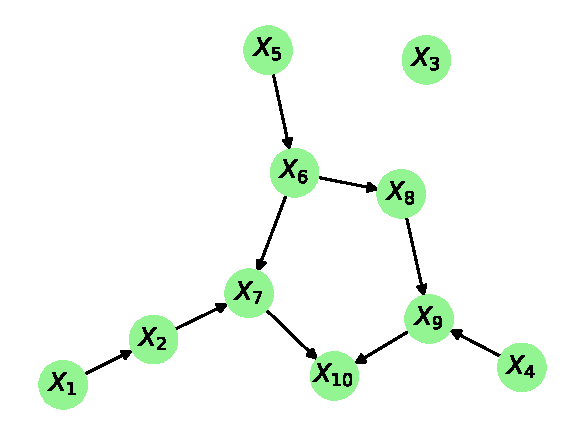
\includegraphics[width=.9\linewidth]{figures/Gaussian Network Theoretical/Graph from triangular G obs - cor.pdf}
        \caption{$G_{dir}$ as a graph}
        % \label{fig:Gaussian 3x3 large s}
    \end{subfigure}
    \caption{For the linear network defined in \autoref{eq:example Gaussian network}, using a triangular $G_{obs}$ (a) with the true topological structure we are able to perfectly rediscover the causal structure as seen in (b) and (c).}
    \label{fig:Gaussian network triangular G_obs using correlation}
\end{figure}

\end{document}